%!TEX program = xelatex
%!TEX root = ../all_beamer.tex

% ============================================================
%  Beamer presentation: Generative Probabilistic Classification
%  Course of Machine Learning – University of Rome "Tor Vergata"
%  Giorgio Gambosi – A.Y. 2025–2026
%  Style modelled on the SLT beamer deck
% ============================================================
%% !TEX root = all_beamer.tex
% ==============================================================================
% HEADER LATEX PER PRESENTAZIONI BEAMER
% Corso di Machine Learning - Giorgio Gambosi
% Università di Roma "Tor Vergata"
% ==============================================================================

% ------------------------------------------------------------------------------
% CLASSE DOCUMENTO E METADATI
% ------------------------------------------------------------------------------
\documentclass[aspectratio=169, 10pt]{beamer}

\subtitle{Course of Machine Learning}
\author{Giorgio Gambosi}
\institute[Tor Vergata]{Master's Degree in Computer Science\\University of Rome ``Tor Vergata''}
\date{A.Y. 2025--2026}

% ------------------------------------------------------------------------------
% PACCHETTI MATEMATICI
% ------------------------------------------------------------------------------
\usepackage{amsmath, amssymb, amsfonts, mathtools, amsthm}
\usepackage{bm}              % Simboli matematici in grassetto
\usepackage{upgreek}         % Lettere greche dritte
\usepackage{derivative}      % Gestione semplificata delle derivate

% ------------------------------------------------------------------------------
% PACCHETTI GRAFICI E VISUALIZZAZIONE
% ------------------------------------------------------------------------------
\usepackage{graphicx}        % Inclusione immagini
\usepackage{xcolor}          % Gestione colori
\usepackage{xkcdcolors}      % Colori aggiuntivi stile xkcd
\usepackage{microtype}       % Miglioramenti tipografici

% ------------------------------------------------------------------------------
% PACCHETTI PER TABELLE
% ------------------------------------------------------------------------------
\usepackage{booktabs}        % Tabelle professionali
\usepackage{array}           % Estensioni per tabelle
\usepackage{multirow}        % Celle multi-riga
\usepackage{multicol}        % Layout multi-colonna

% ------------------------------------------------------------------------------
% TIKZ E PGFPLOTS
% ------------------------------------------------------------------------------
\usepackage{tikz}
\usepackage{tikz-network}
\usepackage[customcolors]{hf-tikz}
\usepackage{pgfplots}
\pgfplotsset{compat=1.18}
\usepgfplotslibrary{fillbetween}

% Librerie TikZ
\usetikzlibrary{arrows, arrows.meta, decorations.pathmorphing, decorations.pathreplacing}
\usetikzlibrary{decorations.markings, snakes, positioning, backgrounds, fit, shadows}
\usetikzlibrary{automata, patterns, calc, intersections, through, shapes}
\usetikzlibrary{shapes.geometric, shapes.arrows, scopes, chains, matrix}

% ------------------------------------------------------------------------------
% ALTRI PACCHETTI
% ------------------------------------------------------------------------------
\usepackage[skins]{tcolorbox}  % Box colorati
\usepackage{subcaption}         % Sottocaption per figure
\usepackage{listings}           % Inclusione codice sorgente

% ------------------------------------------------------------------------------
% TEMA E STILE BEAMER
% ------------------------------------------------------------------------------
\usetheme{Madrid}
\usecolortheme{whale}
\useinnertheme{rounded}
\usefonttheme{professionalfonts}
\setbeamertemplate{navigation symbols}{}  % Rimuove simboli di navigazione

% ------------------------------------------------------------------------------
% DEFINIZIONE COLORI PERSONALIZZATI
% ------------------------------------------------------------------------------
% Colori principali del tema
\definecolor{MainBlue}{RGB}{31,56,100}      % Blu principale (header, titoli)
\definecolor{AccentBlue}{RGB}{70,130,180}   % Blu accento (blocchi)
\definecolor{AlertRed}{RGB}{160,30,30}      % Rosso per alert
\definecolor{ExGreen}{RGB}{30,120,60}       % Verde per esempi
\definecolor{BlockBg}{RGB}{220,232,246}     % Sfondo blocchi
\definecolor{torgray}{RGB}{220,225,235}     % Grigio Tor Vergata

% Colori alternativi (Tor Vergata style)
\definecolor{TvDark}{RGB}{30,50,80}         % Blu scuro header
\definecolor{TvMid}{RGB}{70,100,140}        % Blu medio blocchi
\definecolor{TvLight}{RGB}{210,220,235}     % Blu chiaro sfondi
\definecolor{TvAlert}{RGB}{160,30,30}       % Rosso alert
\definecolor{TvGreen}{RGB}{20,100,50}       % Verde esempi

% Colori supplementari
\definecolor{torred}{RGB}{153,0,0}
\definecolor{torcyan}{RGB}{0,112,192}
\definecolor{cerise}{HTML}{DA3A62}
\definecolor{teal}{HTML}{029386}
\definecolor{slateblue}{HTML}{5B5EA6}
\definecolor{orange}{HTML}{F97306}

% Colori per nodi TikZ
\definecolor{nodeblue}{RGB}{101,140,196}    % xkcd Faded Blue

% ------------------------------------------------------------------------------
% CONFIGURAZIONE COLORI BEAMER
% ------------------------------------------------------------------------------
\setbeamercolor{frametitle}{bg=MainBlue, fg=white}
\setbeamercolor{title}{bg=MainBlue, fg=white}
\setbeamercolor{structure}{fg=MainBlue}

% Blocchi standard
\setbeamercolor{block title}{bg=AccentBlue, fg=white}
\setbeamercolor{block body}{bg=BlockBg}

% Blocchi alert
\setbeamercolor{block title alerted}{bg=AlertRed, fg=white}
\setbeamercolor{block body alerted}{bg=red!8}

% Blocchi esempio
\setbeamercolor{block title example}{bg=ExGreen, fg=white}
\setbeamercolor{block body example}{bg=green!7}

% ------------------------------------------------------------------------------
% CONFIGURAZIONE FONT BEAMER
% ------------------------------------------------------------------------------
\setbeamerfont{frametitle}{size=\normalsize,series=\bfseries}
\setbeamerfont{block title}{size=\small,series=\bfseries}

% ------------------------------------------------------------------------------
% STILI TIKZ PERSONALIZZATI
% ------------------------------------------------------------------------------
\tikzset{
  >=latex,  % Frecce stile LaTeX di default
  % Nodi per reti neurali
  node/.style={thick,circle,draw=myblue,minimum size=22,inner sep=0.5,outer sep=0.6},
  node in/.style={node,green!20!black,draw=mygreen!30!black,fill=mygreen!25},
  node hidden/.style={node,blue!20!black,draw=myblue!30!black,fill=myblue!20},
  node convol/.style={node,orange!20!black,draw=myorange!30!black,fill=myorange!20},
  node out/.style={node,red!20!black,draw=myred!30!black,fill=myred!20},
  % Connessioni
  connect/.style={thick,mydarkblue},
  connect arrow/.style={-{Latex[length=4,width=3.5]},thick,mydarkblue,shorten <=0.5,shorten >=1},
  % Stili numerati per facile mappatura
  node 1/.style={node in},
  node 2/.style={node hidden},
  node 3/.style={node out}
}

% ------------------------------------------------------------------------------
% AMBIENTI TEOREMI
% ------------------------------------------------------------------------------
\setbeamertemplate{theorems}[numbered]
\newtheorem{mytheorem}{Theorem}
\newtheorem{mydefinition}{Definition}

% ------------------------------------------------------------------------------
% CONFIGURAZIONE LISTINGS (CODICE)
% ------------------------------------------------------------------------------
\lstset{
  language=Python,
  basicstyle=\ttfamily\tiny,
  keywordstyle=\color{MainBlue}\bfseries,
  commentstyle=\color{gray},
  frame=single,
  breaklines=true,
}

% ==============================================================================
% MACRO MATEMATICHE PERSONALIZZATE
% ==============================================================================

% ------------------------------------------------------------------------------
% SPAZI CALLIGRAFICI (Calligraphic spaces)
% ------------------------------------------------------------------------------
\providecommand{\calX}{\mathcal{X}}         % Spazio input
\providecommand{\calY}{\mathcal{Y}}         % Spazio output
\providecommand{\calH}{\mathcal{H}}         % Spazio ipotesi
\providecommand{\calT}{\mathcal{T}}         % Training set
\providecommand{\calA}{\mathcal{A}}         % Algoritmo
\providecommand{\calR}{\mathcal{R}}         % Rischio
\providecommand{\calF}{\mathcal{F}}         % Famiglia di funzioni
\providecommand{\calL}{\mathcal{L}}         % Loss function

% Alias per compatibilità
\providecommand{\Rr}{\mathcal{R}}
\providecommand{\Tr}{\mathcal{T}}
\providecommand{\Hr}{\mathcal{H}}

% ------------------------------------------------------------------------------
% RISCHIO E PROBABILITÀ
% ------------------------------------------------------------------------------
\providecommand{\barR}{\overline{\mathcal{R}}}  % Rischio empirico
\providecommand{\EmpR}{\overline{\mathcal{R}}}  % Rischio empirico (alias)
\providecommand{\Rbar}{\overline{\mathcal{R}}}  % Rischio empirico (alias)
\providecommand{\pM}{p_M}                       % Probabilità modello
\providecommand{\pC}{p_C}                       % Probabilità corretta
\providecommand{\Prob}[2]{\mathbb{P}_{#1}\!\left[#2\right]}  % Probabilità

% ------------------------------------------------------------------------------
% FUNZIONI INDICATRICI
% ------------------------------------------------------------------------------
\providecommand{\indicator}[1]{\mathbf{1}\!\left[#1\right]}  % Funzione indicatrice
\providecommand{\ind}[1]{\mathbf{1}[#1]}                      % Versione breve

% ------------------------------------------------------------------------------
% OPERATORI MATEMATICI
% ------------------------------------------------------------------------------
\providecommand{\argmax}{\operatorname*{arg\,max}}  % Argomento del massimo
\providecommand{\argmin}{\operatorname*{arg\,min}}  % Argomento del minimo
\providecommand{\vcd}[1]{\operatorname{VCdim}(#1)} % VC dimension
\providecommand{\defeq}{\stackrel{\text{def}}{=}}  % Definito come

% ------------------------------------------------------------------------------
% VETTORI E MATRICI (Bold Math)
% ------------------------------------------------------------------------------
% Vettori minuscoli
\providecommand{\bx}{\mathbf{x}}            % Vettore x
\providecommand{\bz}{\mathbf{z}}            % Vettore z
\providecommand{\bw}{\mathbf{w}}            % Vettore peso
\providecommand{\btt}{\mathbf{t}}           % Vettore target
\providecommand{\wvec}{\mathbf{w}}          % Vettore peso (alias)
\providecommand{\bth}{\boldsymbol{\theta}}  % Parametro theta

% Matrici maiuscole
\providecommand{\bX}{\mathbf{X}}            % Matrice dati
\providecommand{\bZ}{\mathbf{Z}}            % Matrice Z
\providecommand{\Xmat}{\mathbf{X}}          % Matrice dati (alias)
\providecommand{\Hmat}{\mathbf{H}}          % Matrice H
\providecommand{\Smat}{\mathbf{S}}          % Matrice scatter generica
\providecommand{\bS}{\mathbf{S}}            % Matrice scatter
\providecommand{\Ii}{\mathbf{I}}            % Matrice identità
\providecommand{\bZero}{\mathbf{0}}         % Vettore zero
\providecommand{\bPsi}{\boldsymbol{\Psi}}   % Matrice Psi

% Medie (overline)
\providecommand{\ox}{\overline{\mathbf{x}}} % Media vettore x
\providecommand{\ow}{\overline{\mathbf{w}}} % Media vettore w
\providecommand{\oX}{\overline{\mathbf{X}}} % Media matrice X

% Matrici scatter specifiche (analisi discriminante)
\providecommand{\SW}{\mathbf{S}_W}          % Within-class scatter
\providecommand{\SB}{\mathbf{S}_B}          % Between-class scatter
\providecommand{\ST}{\mathbf{S}_T}          % Total scatter
\providecommand{\GX}{G_{\mathbf{X}}}        % Matrice Gram

% ------------------------------------------------------------------------------
% COMANDI DI FORMATTAZIONE TESTO
% ------------------------------------------------------------------------------
\providecommand{\term}[1]{\textbf{\color{accent}#1}}        % Termine importante
\providecommand{\halert}[1]{{\color{AlertRed}\textbf{#1}}}  % Alert rosso
\providecommand{\mlalert}[1]{{\color{AccentBlue}\textbf{#1}}}  % Alert blu
\providecommand{\mlemph}[1]{{\color{MainBlue}\textit{#1}}}  % Enfasi blu

% ==============================================================================
% FINE HEADER
% ==============================================================================

\newcommand{\blankpage}{
\clearpage
\thispagestyle{empty}
\null
\clearpage
}


%\documentclass[aspectratio=169,t]{beamer}
%
%% ---------- theme & colours ----------
%\usetheme{Madrid}
%\usecolortheme{whale}


%\definecolor{torred}{RGB}{153,0,0}
%\definecolor{torcyan}{RGB}{0,112,192}

%\setbeamercolor{structure}{fg=MainBlue}
%\setbeamercolor{frametitle}{bg=MainBlue,fg=white}
%\setbeamercolor{title}{bg=MainBlue,fg=white}
%\setbeamercolor{block title}{bg=torcyan,fg=white}
%\setbeamercolor{block title alerted}{bg=torred,fg=white}
%\setbeamercolor{block title example}{bg=MainBlue!60!black,fg=white}
%\setbeamercolor{alerted text}{fg=torred}
%
%\setbeamerfont{frametitle}{size=\normalsize,series=\bfseries}
%\setbeamerfont{block title}{size=\small,series=\bfseries}

% ---------- packages ----------
%\usepackage{amsmath,amssymb,bm}
%\usepackage{mathtools}
%\usepackage{booktabs}
%\usepackage{graphicx}
%\usepackage{tikz}
%\usetikzlibrary{arrows.meta,shapes,positioning}

% ---------- convenience macros ----------
%\newcommand{\x}{\mathbf{x}}
%\newcommand{\w}{\mathbf{w}}
%\newcommand{\I}{\mathbf{I}}
%\newcommand{\Zero}{\mathbf{0}}
%\newcommand{\Vmu}{\boldsymbol{\mu}}
%\newcommand{\VSigma}{\boldsymbol{\Sigma}}
%\newcommand{\Vphi}{\boldsymbol{\phi}}
%\newcommand{\Valpha}{\boldsymbol{\alpha}}
%\newcommand{\vnorm}[1]{\|#1\|}
%\newcommand{\ev}[2]{\mathbb{E}_{#1}\!\left[#2\right]}
%\newcommand{\argmax}{\operatorname{arg\,max}}

% ---------- title info ----------
\title{Generative Probabilistic Classification}
%\subtitle{Course of Machine Learning}
%\author{Giorgio Gambosi}
%\institute{Master's Degree in Computer Science\\University of Rome ``Tor Vergata''}
%\date{A.Y.\ 2025--2026}

% ============================================================
%\begin{document}
% ============================================================

\begin{frame}
  \titlepage
\end{frame}

% ---------- outline ----------
\begin{frame}{Outline}
  \tableofcontents
\end{frame}

% ============================================================
\section{Introduction to Generative Models}
% ============================================================

\begin{frame}{Discriminative vs.\ Generative Approaches}
  \begin{block}{Discriminative viewpoint (so far)}
    \begin{itemize}
      \item Focus: learn the decision boundary or posterior $p(C_k\mid\x)$ directly.
      \item Examples: logistic regression, SVMs.
    \end{itemize}
  \end{block}

  \begin{alertblock}{Generative viewpoint (this chapter)}
    \begin{itemize}
      \item Focus: model \emph{how data in each class are produced}.
      \item Each class $C_k$ is described by a class-conditional distribution $p(\x\mid C_k)$.
      \item If $p(\x\mid C_k)$ is known, we can \textbf{generate} realistic samples of class $C_k$.
    \end{itemize}
  \end{alertblock}

  \begin{block}{Key analogy}
    Language models learned for text classification can be used to \emph{generate} new documents
    statistically similar to a training corpus — the same idea applies here.
  \end{block}
\end{frame}

% --------------------------------------------------------
\begin{frame}{Components of a Generative Model}
  \begin{block}{Two main ingredients}
    \begin{itemize}
      \item \textbf{Class-conditional distribution} $p(\x\mid C_k)$: captures the typical variability
            of samples in class $C_k$.
      \item \textbf{Class prior} $p(C_k)$: probability of observing class $C_k$ before seeing any data.
            Encodes global information (e.g.\ class imbalance).
    \end{itemize}
  \end{block}

  \begin{block}{Classification via Bayes' rule}
    Posterior probabilities are obtained directly:
    \[
      p(C_k\mid\x)=\frac{p(\x\mid C_k)\,p(C_k)}{\sum_j p(\x\mid C_j)\,p(C_j)}.
    \]
    \begin{itemize}
      \item Parameters of $p(\x\mid C_k)$ and $p(C_k)$: learned by \textbf{maximum likelihood}.
      \item Classification: assign $\x$ to $\argmax_k\; p(C_k\mid\x)$.
    \end{itemize}
  \end{block}
\end{frame}

% ============================================================
\section{Posterior Probabilities: Binary and Multiclass Cases}
% ============================================================

\begin{frame}{Deriving Posterior Probabilities — Binary Case}
  \begin{block}{Setup}
    Two classes $C_1$, $C_2$.  Apply Bayes' rule:
    \[
      p(C_1\mid\x)=\frac{p(\x\mid C_1)\,p(C_1)}{p(\x\mid C_1)\,p(C_1)+p(\x\mid C_2)\,p(C_2)}
      =\frac{1}{1+\dfrac{p(\x\mid C_2)\,p(C_2)}{p(\x\mid C_1)\,p(C_1)}}.
    \]
  \end{block}

  \begin{block}{Log-odds (log odds ratio)}
    Define the \alert{log odds}:
    \[
      a(\x)=\log\frac{p(\x\mid C_1)\,p(C_1)}{p(\x\mid C_2)\,p(C_2)}
      =\log\frac{p(C_1\mid\x)}{p(C_2\mid\x)}.
    \]
    \begin{itemize}
      \item Turns multiplicative comparisons into additive ones.
      \item Simplifies algebra and optimization.
    \end{itemize}
  \end{block}
\end{frame}

% --------------------------------------------------------
\begin{frame}{The Sigmoid Function}
  \begin{block}{Sigmoid form of posterior}
    Substituting $a(\x)$ into the Bayes formula:
    \[
      p(C_1\mid\x)=\frac{1}{1+e^{-a(\x)}}=\sigma(a(\x)),
      \qquad
      p(C_2\mid\x)=\frac{1}{1+e^{a(\x)}}.
    \]
    \textbf{The sigmoid arises naturally from Bayes' rule.}
  \end{block}

  \begin{columns}[T]
    \begin{column}{0.48\textwidth}
      \begin{block}{Key properties of $\sigma$}
        \begin{itemize}
          \item Smooth map $\mathbb{R}\to(0,1)$.
          \item $\sigma(-x)=1-\sigma(x)$ — class symmetry.
          \item $\dfrac{d\sigma(x)}{dx}=\sigma(x)(1-\sigma(x))$ — compact derivative.
        \end{itemize}
      \end{block}
    \end{column}
    \begin{column}{0.48\textwidth}
      \begin{block}{Interpretation}
        \begin{itemize}
          \item $a(\x)\gg 0$: confident prediction for $C_1$.
          \item $a(\x)\ll 0$: confident prediction for $C_2$.
          \item $a(\x)=0$: equal posteriors — decision boundary.
        \end{itemize}
      \end{block}
    \end{column}
  \end{columns}
\end{frame}

% --------------------------------------------------------
\begin{frame}{Sigmoid — Graphical View}
  \begin{center}
    % Placeholder for Figure4-9.pdf (sigmoid curve)
    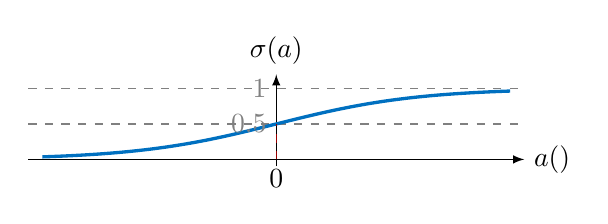
\begin{tikzpicture}[scale=0.9]
      \draw[->] (-3.5,0)--(3.5,0) node[right]{$a(\x)$};
      \draw[->] (0,-0.1)--(0,1.2) node[above]{$\sigma(a)$};
      \draw[dashed,gray] (-3.5,1)--(3.5,1);
      \draw[dashed,gray] (-3.5,0.5)--(3.5,0.5);
      \draw[very thick,torcyan,domain=-3.3:3.3,smooth,samples=80]
        plot(\x,{1/(1+exp(-\x))});
      \node[below right,gray] at (3.5,0) {};
      \node[left,gray] at (0,1){$1$};
      \node[left,gray] at (0,0.5){$0.5$};
      \draw[dashed,torred] (0,0)--(0,0.5);
      \node[below] at (0,0){$0$};
    \end{tikzpicture}
  \end{center}
  \vspace{-2mm}
  {\small The sigmoid provides a smooth mapping from the unconstrained log-odds
  $a(\x)\in\mathbb{R}$ to a valid probability in $(0,1)$.}
\end{frame}

% --------------------------------------------------------
\begin{frame}{Deriving Posterior Probabilities — Multiclass Case}
  \begin{block}{$K>2$ classes: softmax}
    Bayes' rule gives:
    \[
      p(C_k\mid\x)=\frac{p(\x\mid C_k)\,p(C_k)}{\sum_j p(\x\mid C_j)\,p(C_j)}.
    \]
    Define unnormalized log-posteriors:
    \[
      a_k(\x)=\log(p(\x\mid C_k)\,p(C_k))=\log p(\x\mid C_k)+\log p(C_k).
    \]
    Then:
    \[
      p(C_k\mid\x)=\frac{e^{a_k}}{\sum_j e^{a_j}}=s(a_k).
    \]
  \end{block}

  \begin{block}{Softmax function}
    \begin{itemize}
      \item Extends sigmoid to the multiclass setting.
      \item Converts a vector of real scores into a probability distribution.
      \item Smoothed version of $\max$: differentiable everywhere.
      \item If one score $a_k\gg$ all others: $s(a_k)\approx 1$.
    \end{itemize}
  \end{block}
\end{frame}

% ============================================================
\section{Gaussian Discriminant Analysis (GDA)}
% ============================================================

\begin{frame}{GDA — Shared Covariance Hypothesis}
  \begin{block}{Gaussian class-conditional distributions}
    Assume all classes share the same covariance matrix $\VSigma$ ($d\times d$):
    \[
      p(\x\mid C_k)=\mathcal{N}(\x\mid\Vmu_k,\VSigma).
    \]
    \begin{itemize}
      \item $\Vmu_k$: center (mean) of class $C_k$.
      \item $\VSigma$: shared spread and correlation structure.
    \end{itemize}
  \end{block}

  \begin{alertblock}{Why GDA?}
    \begin{itemize}
      \item Gaussian assumption: reasonable for real-valued features after preprocessing.
      \item Leads to \textbf{analytically derived} posteriors with clear geometric interpretation.
      \item Shared covariance $\Rightarrow$ \textbf{linear decision boundaries}.
    \end{itemize}
  \end{alertblock}
\end{frame}

% --------------------------------------------------------
\begin{frame}{GDA — Linear Discriminant (Binary Case)}
  \begin{block}{Log-odds under shared-covariance GDA}
    The Gaussian quadratic terms \textbf{cancel} in the log ratio, leaving:
    \[
      a(\x)=\w^T\x+b,
    \]
    with
    \[
      \w=\VSigma^{-1}(\Vmu_1-\Vmu_2),
      \qquad
      b=\tfrac{1}{2}\!\left(\Vmu_2^T\VSigma^{-1}\Vmu_2
           -\Vmu_1^T\VSigma^{-1}\Vmu_1\right)+\log\frac{p(C_1)}{p(C_2)}.
    \]
  \end{block}

  \begin{block}{Posterior}
    \[
      p(C_1\mid\x)=\sigma(\w^T\x+b).
    \]
    \begin{itemize}
      \item Non-linear function applied to a \textbf{linear combination} of features.
      \item This is the structure of a \alert{generalized linear model}.
      \item Despite the probabilistic derivation, the model is identical in form to
            logistic regression.
    \end{itemize}
  \end{block}
\end{frame}

% --------------------------------------------------------
\begin{frame}{GDA — Decision Boundary (Binary Case)}
  \begin{block}{Decision boundary}
    The classifier is indifferent when $p(C_1\mid\x)=p(C_2\mid\x)$, i.e.\ $a(\x)=0$:
    \[
      \w^T\x+b=0.
    \]
    Explicitly:
    \[
      \VSigma^{-1}(\Vmu_1-\Vmu_2)\,\x
      +\tfrac{1}{2}\!\left(\Vmu_2^T\VSigma^{-1}\Vmu_2-\Vmu_1^T\VSigma^{-1}\Vmu_1\right)
      +\log\frac{p(C_2)}{p(C_1)}=0.
    \]
  \end{block}

  \begin{block}{Observations}
    \begin{itemize}
      \item The separating \textbf{hyperplane} depends on class means, covariance, and priors.
      \item Changing priors shifts the boundary (via the bias term).
      \item Isotropic case $\VSigma=\lambda\I$: boundary determined by the difference of class means.
    \end{itemize}
  \end{block}
\end{frame}

% --------------------------------------------------------
\begin{frame}{GDA — Example (Linear Boundary)}
  \begin{columns}[c]
    \begin{column}{0.48\textwidth}
      \centering
      % Placeholder for classcond2.pdf
      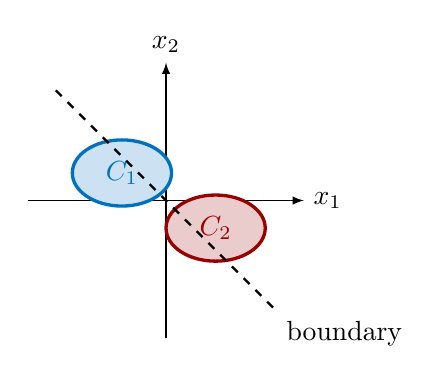
\begin{tikzpicture}[scale=0.7]
        \draw[->](-2.5,0)--(2.5,0) node[right]{$x_1$};
        \draw[->](0,-2.5)--(0,2.5) node[above]{$x_2$};
        % Class 1 ellipse
        \draw[very thick,torcyan,fill=torcyan!20]
          (-0.8,0.5) ellipse (0.9cm and 0.6cm);
        \node[torcyan] at (-0.8,0.5) {$C_1$};
        % Class 2 ellipse
        \draw[very thick,torred,fill=torred!20]
          (0.9,-0.5) ellipse (0.9cm and 0.6cm);
        \node[torred] at (0.9,-0.5) {$C_2$};
        % Decision boundary
        \draw[thick,black,dashed](-2,2)--(2,-2) node[below right,black]{boundary};
      \end{tikzpicture}\\
      \small Class-conditional distributions $p(\x|C_k)$
    \end{column}
    \begin{column}{0.48\textwidth}
      \centering
      % Placeholder for postprob2.pdf
      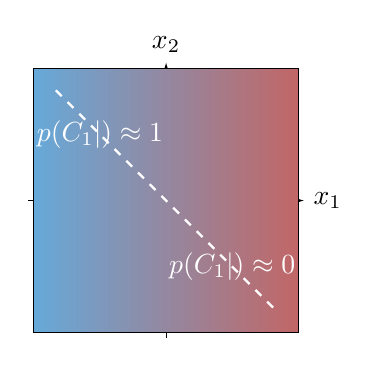
\begin{tikzpicture}[scale=0.7]
        \draw[->](-2.5,0)--(2.5,0) node[right]{$x_1$};
        \draw[->](0,-2.5)--(0,2.5) node[above]{$x_2$};
        \shadedraw[left color=torcyan!60, right color=torred!60]
          (-2.4,-2.4) rectangle (2.4,2.4);
        \draw[thick,white,dashed](-2,2)--(2,-2);
        \node[white] at (-1.2,1.2) {$p(C_1|\x)\approx1$};
        \node[white] at (1.2,-1.2) {$p(C_1|\x)\approx0$};
      \end{tikzpicture}\\
      \small Posterior $p(C_1|\x)$: sigmoidal transition
    \end{column}
  \end{columns}
  \vspace{2mm}
  {\small Left: class-conditional Gaussians in $d=2$. Right: posterior probability
  $p(C_1|\x)$ showing the characteristic sigmoidal transition across the decision boundary.}
\end{frame}

% --------------------------------------------------------
\begin{frame}{GDA — Multiple Classes ($K>2$)}
  \begin{block}{Multiclass posteriors}
    \[
      p(C_k\mid\x)=s\bigl(\w_k^T\x+b_k\bigr),
    \]
    where under shared-covariance GDA:
    \[
      \w_k=\VSigma^{-1}\Vmu_k,\qquad
      b_k=-\tfrac{1}{2}\Vmu_k^T\VSigma^{-1}\Vmu_k+\log p(C_k)+\text{const.}
    \]
  \end{block}

  \begin{block}{Decision boundaries}
    \begin{itemize}
      \item A point $\x$ lies on the boundary between $C_j$ and $C_k$ when
            $a_j(\x)=a_k(\x)$ (equal posteriors).
      \item Since both $a_j$ and $a_k$ are \textbf{affine} in $\x$, their equality defines a hyperplane.
      \item All pairwise boundaries are hyperplanes $\Rightarrow$ \textbf{linear multiclass classifier}.
    \end{itemize}
  \end{block}
\end{frame}

% --------------------------------------------------------
\begin{frame}{GDA — General (Unequal) Covariance Matrices}
  \begin{block}{Relaxing the shared covariance}
    Allow each class to have its own covariance $\VSigma_k$.  The log-odds become:
    \[
      a(\x)=\tfrac{1}{2}\!\left[(\x-\Vmu_2)^T\VSigma_2^{-1}(\x-\Vmu_2)
            -(\x-\Vmu_1)^T\VSigma_1^{-1}(\x-\Vmu_1)\right]
            +\tfrac{1}{2}\log\frac{|\VSigma_2|}{|\VSigma_1|}
            +\log\frac{p(C_1)}{p(C_2)}.
    \]
  \end{block}

  \begin{block}{Quadratic boundary}
    \begin{itemize}
      \item Quadratic terms in $\x$ do \textbf{not} cancel.
      \item Decision boundary: at most a \textbf{quadratic surface} (conic section in 2D).
      \item Each Gaussian can have its own shape and orientation.
      \item \textbf{Quadratic Discriminant Analysis (QDA)}.
    \end{itemize}
  \end{block}
\end{frame}

% --------------------------------------------------------
\begin{frame}{QDA — Example (Curved Boundaries)}
  \begin{columns}[c]
    \begin{column}{0.48\textwidth}
      \centering
      % Placeholder for quadgda1.pdf
      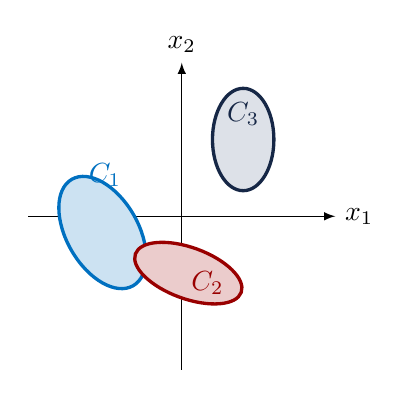
\begin{tikzpicture}[scale=0.65]
        \draw[->](-3,0)--(3,0) node[right]{$x_1$};
        \draw[->](0,-3)--(0,3) node[above]{$x_2$};
        \draw[very thick,torcyan,fill=torcyan!20,rotate=30]
          (-1.5,0.5) ellipse (0.7cm and 1.2cm);
        \node[torcyan] at (-1.5,0.8){$C_1$};
        \draw[very thick,torred,fill=torred!20,rotate=-20]
          (0.5,-1) ellipse (1.1cm and 0.5cm);
        \node[torred] at (0.5,-1.3){$C_2$};
        \draw[very thick,MainBlue!70!black,fill=MainBlue!15]
          (1.2,1.5) ellipse (0.6cm and 1.0cm);
        \node[MainBlue!70!black] at (1.2,2.0){$C_3$};
      \end{tikzpicture}\\
      \small Three Gaussians with different covariances
    \end{column}
    \begin{column}{0.48\textwidth}
      \centering
      % Placeholder for quadgda2.pdf
      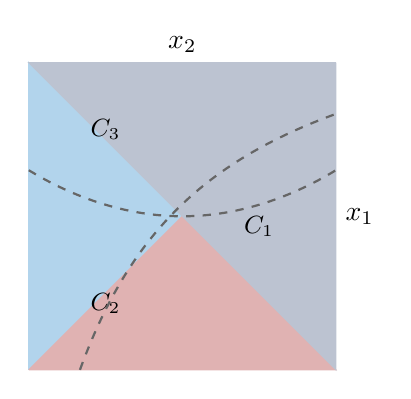
\begin{tikzpicture}[scale=0.65]
        \draw[->](-3,0)--(3,0) node[right]{$x_1$};
        \draw[->](0,-3)--(0,3) node[above]{$x_2$};
        \filldraw[torcyan!30](-3,-3)--(-3,3)--(0,0)--(-3,-3);
        \filldraw[torred!30](-3,-3)--(3,-3)--(0,0)--(-3,-3);
        \filldraw[MainBlue!30](3,3)--(-3,3)--(0,0)--(3,-3)--(3,3);
        \draw[thick,black!60,dashed](-3,0.9) parabola bend(0,0) (3,0.9);
        \draw[thick,black!60,dashed](-2,-3) to[out=70,in=200] (3,2);
        \node at (-1.5,1.7){\small $C_3$};
        \node at (-1.5,-1.7){\small $C_2$};
        \node at (1.5,-0.2){\small $C_1$};
      \end{tikzpicture}\\
      \small Curved (quadratic) decision surfaces
    \end{column}
  \end{columns}
  \vspace{2mm}
  {\small Left: three classes with different covariance matrices.
   Right: posterior class regions separated by curved quadratic boundary surfaces.}
\end{frame}

% ============================================================
\section{Maximum Likelihood Estimation in GDA}
% ============================================================

\begin{frame}{GDA Parameter Estimation — Setup}
  \begin{block}{Goal}
    Learn $\Vmu_1, \Vmu_2, \VSigma, \pi=p(C_1)$ from training data
    $\mathcal{T}=\{(\x_i,t_i)\}_{i=1}^n$, with $t_i\in\{0,1\}$.
  \end{block}

  \begin{block}{Joint data model}
    \begin{align*}
      p(\x,C_1)&=\pi\cdot\mathcal{N}(\x\mid\Vmu_1,\VSigma),\\
      p(\x,C_2)&=(1-\pi)\cdot\mathcal{N}(\x\mid\Vmu_2,\VSigma).
    \end{align*}
  \end{block}

  \begin{block}{Log-likelihood}
    \[
      l(\pi,\Vmu_1,\Vmu_2,\VSigma\mid\mathcal{T})
      =\sum_{i=1}^n \bigl[t_i\log\pi + t_i\log\mathcal{N}(\x_i|\Vmu_1,\VSigma)\bigr]
       +\sum_{i=1}^n \bigl[(1-t_i)\log(1-\pi)+(1-t_i)\log\mathcal{N}(\x_i|\Vmu_2,\VSigma)\bigr].
    \]
  \end{block}
\end{frame}

% --------------------------------------------------------
\begin{frame}{GDA ML Estimates — Closed-Form Solutions}
  \begin{block}{MLE results}
    Setting gradients to zero yields:

    \medskip
    \begin{tabular}{ll}
      \toprule
      \textbf{Parameter} & \textbf{MLE} \\
      \midrule
      Class prior $\hat\pi$ & $n_1/n$ \quad (empirical class frequency)\\[4pt]
      Class means $\hat\Vmu_k$ & $\dfrac{1}{n_k}\displaystyle\sum_{\x_i\in C_k}\x_i$
                                  \quad (sample mean of class $k$)\\[8pt]
      Shared covariance $\hat\VSigma$ & $\dfrac{n_1}{n}S_1+\dfrac{n_2}{n}S_2$
                                         \quad (weighted average of within-class covariances)\\
      \bottomrule
    \end{tabular}
  \end{block}

  \begin{block}{Within-class covariances}
    \[
      S_k=\frac{1}{n_k}\sum_{\x_i\in C_k}(\x_i-\hat\Vmu_k)(\x_i-\hat\Vmu_k)^T.
    \]
    \begin{itemize}
      \item $\hat\VSigma$ captures the pooled spread around class centers.
      \item All estimates have natural statistical interpretations.
    \end{itemize}
  \end{block}
\end{frame}

% ============================================================
\section{MAP Estimation and Regularization}
% ============================================================

\begin{frame}{From ML to MAP Estimation}
  \begin{block}{Motivation}
    \begin{itemize}
      \item ML estimates can be unstable: ill-conditioned $\hat\VSigma$ when $d$ is large relative to $n$.
      \item MAP = maximize posterior $p(\theta\mid\mathcal{T})\propto p(\mathcal{T}\mid\theta)p(\theta)$.
    \end{itemize}
  \end{block}

  \begin{block}{MAP objective}
    \[
      \hat\theta_{\mathrm{MAP}}=\argmax_\theta\;\bigl[\log p(\mathcal{T}\mid\theta)+\underbrace{\log p(\theta)}_{\text{regularization}}\bigr].
    \]
  \end{block}

  \begin{alertblock}{Interpretation}
    \begin{itemize}
      \item The prior $\log p(\theta)$ acts as a \textbf{regularization term}.
      \item Large data: likelihood dominates, MAP $\approx$ ML.
      \item Small data / high dimension: prior has decisive influence.
    \end{itemize}
  \end{alertblock}
\end{frame}

% --------------------------------------------------------
\begin{frame}{MAP for Class Prior — Beta Prior}
  \begin{block}{Beta prior on $\pi=p(C_1)$}
    \[
      \pi\sim\mathrm{Beta}(\alpha,\beta)\quad\Rightarrow\quad
      p(\pi\mid\mathcal{T})\propto\pi^{n_1+\alpha-1}(1-\pi)^{n_2+\beta-1}.
    \]
    \begin{itemize}
      \item Posterior: Beta with updated parameters.
      \item MAP estimate: smoothed frequency, with prior contributing \textbf{pseudo-counts}
            $(\alpha-1)$ and $(\beta-1)$.
      \item Prevents $\hat\pi$ from collapsing to $0$ or $1$ with small or unbalanced datasets.
    \end{itemize}
  \end{block}
\end{frame}

% --------------------------------------------------------
\begin{frame}{MAP for Covariance — Shrinkage}
  \begin{block}{The problem with ML covariance}
    \begin{itemize}
      \item In high dimension: $\hat\VSigma_{\mathrm{ML}}$ can be \textbf{ill-conditioned or singular}.
      \item Small eigenvalues $\to$ huge inverse eigenvalues $\to$ unstable discriminant direction $\w$.
    \end{itemize}
  \end{block}

  \begin{block}{MAP solution — Shrinkage}
    With an inverse-Wishart prior, the MAP estimate interpolates between the sample covariance
    and a structured target:
    \[
      \hat\VSigma_{\mathrm{MAP}}\approx(1-\lambda)\,\hat\VSigma_{\mathrm{ML}}+\lambda\,\tau\I,
      \qquad\lambda\in[0,1],\;\tau>0.
    \]
    \begin{itemize}
      \item $\lambda$ large (few data): estimate closer to $\tau\I$ — stable inversion.
      \item $\lambda$ small (many data): estimate approaches $\hat\VSigma_{\mathrm{ML}}$.
      \item \textbf{Effect}: eigenvalues pulled toward a common scale; spurious correlations damped.
    \end{itemize}
  \end{block}
\end{frame}

% --------------------------------------------------------
\begin{frame}{MAP for Class Means — Shrinkage toward Prior}
  \begin{block}{Gaussian prior on $\Vmu_k$}
    \[
      \Vmu_k\sim\mathcal{N}(\Vmu_0,\VSigma_0).
    \]
    Posterior MAP estimate (conjugate prior case):
    \[
      \hat\Vmu_k^{\mathrm{MAP}}=\alpha_k\,\hat\Vmu_k^{\mathrm{ML}}+(1-\alpha_k)\,\Vmu_0,
      \qquad\alpha_k\in(0,1).
    \]
    \begin{itemize}
      \item $\alpha_k\to1$ as $n_k\to\infty$: MAP $\approx$ sample mean.
      \item Small $n_k$: estimate pulled toward prior center $\Vmu_0$.
      \item Reduces risk of fitting noisy class centroids.
    \end{itemize}
  \end{block}

  \begin{alertblock}{Summary}
    MAP provides a principled way to control variance in parameter estimates,
    improving both numerical stability and generalization in finite-sample regimes.
  \end{alertblock}
\end{frame}

% ============================================================
\section{Naive Bayes and Conditional Independence}
% ============================================================

\begin{frame}{Naive Bayes as a General Independence Assumption}
  \begin{block}{Naive Bayes hypothesis}
    Conditioned on the class $C_k$, features are \textbf{mutually independent}:
    \[
      p(\x\mid C_k)=\prod_{i=1}^m p(x_i\mid C_k).
    \]
    \begin{itemize}
      \item Works for \emph{any} feature type: continuous, discrete, or mixed.
      \item Each marginal $p(x_i\mid C_k)$ can belong to any parametric family.
    \end{itemize}
  \end{block}

  \begin{block}{Relation to GDA}
    \begin{itemize}
      \item Continuous features with Gaussian marginals:
            $p(x_i\mid C_k)=\mathcal{N}(x_i\mid\mu_{ki},\sigma_{ki}^2)$.
      \item This is GDA with a \textbf{diagonal} covariance matrix $\VSigma_k$.
      \item Naive Bayes $\equiv$ restricted GDA (inter-feature correlations ignored).
    \end{itemize}
  \end{block}
\end{frame}

% --------------------------------------------------------
\begin{frame}{Naive Bayes — Trade-off}
  \begin{columns}[T]
    \begin{column}{0.48\textwidth}
      \begin{block}{Advantages}
        \begin{itemize}
          \item Drastically fewer parameters: $O(m)$ instead of $O(m^2)$.
          \item Highly beneficial in high-dimensional settings.
          \item Robust when training data is limited.
          \item Fast to train and evaluate.
        \end{itemize}
      \end{block}
    \end{column}
    \begin{column}{0.48\textwidth}
      \begin{alertblock}{Disadvantages}
        \begin{itemize}
          \item Cannot capture \textbf{correlations} between features.
          \item The independence assumption is often violated in practice.
          \item Sacrifices representational richness.
        \end{itemize}
      \end{alertblock}
    \end{column}
  \end{columns}

  \vspace{4mm}
  \begin{exampleblock}{Practical performance}
    Despite the ``naive'' assumption, Naive Bayes often performs \textbf{surprisingly well},
    especially in high-dimensional feature spaces (e.g.\ text classification).
  \end{exampleblock}
\end{frame}

% ============================================================
\section{Language Models for Discrete Features}
% ============================================================

\begin{frame}{Language Models — Definition}
  \begin{block}{What is a language model?}
    \begin{itemize}
      \item A \alert{categorical probability distribution} over a vocabulary $\mathcal{D}=\{t_1,\ldots,t_n\}$.
      \item Vocabulary: constructed from a large, representative corpus.
    \end{itemize}
  \end{block}

  \begin{block}{Bag-of-Words hypothesis}
    \begin{itemize}
      \item Treat each term occurrence as an \textbf{independent event}.
      \item Ignore syntactic, grammatical, and sequential context.
      \item Computationally efficient; captures the document's ``theme''.
      \item Can be used \textbf{generatively}: sampling from the distribution yields
            statistically representative (if syntactically incoherent) documents.
    \end{itemize}
  \end{block}
\end{frame}

% --------------------------------------------------------
\begin{frame}{Constructing the Language Model}
  \begin{block}{Pipeline}
    \begin{enumerate}
      \item \textbf{Vocabulary extraction and pre-processing}
        \begin{itemize}
          \item \alert{Stop word removal}: discard high-frequency, semantically weak words.
          \item \alert{Stemming}: map morphological variants to a common root
                (e.g.\ ``connected'', ``connecting'', ``connection'' $\to$ ``connect'').
        \end{itemize}
      \item \textbf{Compute multiplicities} $m_i$: number of occurrences of $t_i$ in corpus $\mathcal{C}$.
      \item \textbf{Estimate probability vector} $\hat\Vphi=(\hat\phi_1,\ldots,\hat\phi_n)^T$:
        \[
          \hat\phi_i = p(t_i\mid\mathcal{C})=\frac{m_i}{N},\qquad N=\sum_{j=1}^n m_j.
        \]
    \end{enumerate}
  \end{block}

  \begin{block}{Validity constraints}
    \[
      0\le\hat\phi_i\le1\quad\forall\,i,\qquad\sum_{i=1}^n\hat\phi_i=1.
    \]
    $\hat\phi_i$ is the \textbf{Maximum Likelihood Estimate} (MLE) for the probability of $t_i$.
  \end{block}
\end{frame}

% ============================================================
\section{Handling Data Sparsity: Smoothing}
% ============================================================

\begin{frame}{The Zero-Frequency Problem}
  \begin{alertblock}{Problem}
    If a term $t_{\mathrm{new}}$ is absent from $\mathcal{C}$ (i.e.\ $m_{\mathrm{new}}=0$):
    \[
      \hat\phi_{\mathrm{new}}=\frac{0}{N}=0.
    \]
    In classification, a single zero probability kills the entire likelihood product.
    This is an unrealistic ``impossible event'' assignment.
  \end{alertblock}

  \begin{block}{Solution: Smoothing}
    Redistribute probability mass from frequent to unseen terms to ensure
    no term is ever assigned zero probability.
  \end{block}
\end{frame}

% --------------------------------------------------------
\begin{frame}{Laplace (Add-One) Smoothing}
  \begin{block}{Idea}
    Pretend every term in $\mathcal{D}$ has been seen \textbf{at least once more} than observed.
  \end{block}

  \begin{block}{Laplace smoothed estimate}
    \[
      \phi_i^{\mathrm{Lap}}=\frac{m_i+1}{N+n},\qquad n=|\mathcal{D}|.
    \]
    Normalization is preserved:
    \[
      \sum_{i=1}^n\phi_i^{\mathrm{Lap}}=\frac{N+n}{N+n}=1.\quad\checkmark
    \]
  \end{block}

  \begin{block}{Interpretations}
    \begin{itemize}
      \item \textbf{Bayesian}: equivalent to a uniform Dirichlet prior ($\alpha_i=1$ for all $i$).
      \item \textbf{Pseudo-counts}: treats every word as having been seen once before training.
      \item Large corpus ($N\gg n$): smoothing is negligible — MLE dominates.
      \item Small corpus or rare terms: vital safety net.
    \end{itemize}
  \end{block}
\end{frame}

% --------------------------------------------------------
\begin{frame}{Lidstone Smoothing — Generalization}
  \begin{block}{Lidstone's Law}
    Replace ``add one'' with ``add $\alpha$'':
    \[
      \phi_i^{(\alpha)}=\frac{m_i+\alpha}{N+\alpha n},\qquad 0<\alpha\le1.
    \]
    \begin{itemize}
      \item $\alpha=1$: Laplace smoothing.
      \item Small $\alpha$ (e.g.\ $0.1$): less aggressive redistribution, preferred for large-scale NLP.
    \end{itemize}
  \end{block}
\end{frame}

% ============================================================
\section{Bayesian Language Modeling}
% ============================================================

\begin{frame}{Bayesian Framework — Dirichlet-Multinomial Model}
  \begin{block}{Dirichlet prior}
    Treat $\Vphi$ as a random variable.  The conjugate prior for a multinomial is the Dirichlet:
    \[
      p(\phi_1,\ldots,\phi_n\mid\Valpha)
      =\frac{1}{\Delta(\Valpha)}\prod_{i=1}^n\phi_i^{\alpha_i-1},
      \qquad\Valpha=(\alpha_1,\ldots,\alpha_n).
    \]
    \begin{itemize}
      \item $\alpha_i$: ``pseudo-counts'' — prior belief about how often $t_i$ occurs.
    \end{itemize}
  \end{block}

  \begin{block}{Posterior update}
    After observing corpus $\mathcal{C}$ with counts $m_1,\ldots,m_n$:
    \[
      p(\Vphi\mid\mathcal{C},\Valpha)=\mathrm{Dir}\!\left(\Vphi\mid\bar\Valpha\right),
      \qquad\bar\alpha_i=\alpha_i+m_i.
    \]
    Simply \textbf{add observed counts to prior pseudo-counts}.
    Conjugacy guarantees the posterior stays Dirichlet.
  \end{block}
\end{frame}

% --------------------------------------------------------
\begin{frame}{Bayesian Predictive Posterior}
  \begin{block}{Predictive distribution}
    Integrate over $\Vphi$ to obtain the posterior predictive:
    \[
      \hat\phi_j=p(t_j\mid\mathcal{C},\Valpha)
      =\int\phi_j\,\mathrm{Dir}(\Vphi\mid\bar\Valpha)\,d\Vphi
      =\mathbb{E}_{\Vphi\sim\mathrm{Dir}(\cdot\mid\bar\Valpha)}[\phi_j]
      =\frac{\bar\alpha_j}{\sum_k\bar\alpha_k}
      =\frac{\alpha_j+m_j}{\alpha_0+N},
    \]
    where $\alpha_0=\sum_k\alpha_k$ and $N$ is the total corpus size.
  \end{block}

  \begin{block}{Dirichlet smoothing}
    \begin{itemize}
      \item $\alpha_j>0$ ensures $\hat\phi_j>0$ even if $m_j=0$: zero-frequency problem solved.
      \item \textbf{Symmetric prior} $\alpha_i=\alpha$ for all $i$:
        \[
          p(t_j\mid\mathcal{C},\Valpha)=\frac{m_j+\alpha}{\alpha|\mathcal{D}|+N}.
        \]
      \item \textbf{$\alpha=1$}: identical to Laplace smoothing.
    \end{itemize}
  \end{block}
\end{frame}

% ============================================================
\section{Naive Bayes Text Classifier}
% ============================================================

\begin{frame}{Naive Bayes for Document Classification — Setup}
  \begin{block}{Problem}
    Binary classification: $C_1$ vs.\ $C_2$ (e.g.\ Spam/Ham, Positive/Negative sentiment).
    For each document $d$, compute $p(C_k\mid d)$ and assign to the most probable class.
  \end{block}

  \begin{block}{Bayes' rule}
    \[
      p(C_k\mid d)\propto p(d\mid C_k)\,p(C_k).
    \]
    Two components to estimate:
    \begin{enumerate}
      \item \textbf{Prior} $p(C_k)$: ML estimate $=|\mathcal{C}_k|/(|\mathcal{C}_1|+|\mathcal{C}_2|)$.
      \item \textbf{Likelihood} $p(d\mid C_k)$: complex due to sequential word dependencies.
    \end{enumerate}
  \end{block}
\end{frame}

% --------------------------------------------------------
\begin{frame}{Naive Bayes Assumption for Text}
  \begin{block}{Bag-of-Words representation}
    Document $d$ is a multiset of $n_d$ terms:
    $d=\{\bar t_1,\bar t_2,\ldots,\bar t_{n_d}\}$.
  \end{block}

  \begin{alertblock}{Naive Bayes assumption}
    Terms in $d$ are \textbf{pairwise conditionally independent} given $C_k$:
    \[
      p(d\mid C_k)=\prod_{j=1}^{n_d}p(\bar t_j\mid C_k).
    \]
    \begin{itemize}
      \item Ignores linguistic dependencies (``San'' $\to$ ``Francisco'').
      \item Dramatically simplifies computation.
      \item Individual probabilities $p(\bar t_j\mid C_k)$: from the class language models.
      \item Smoothing prevents the product from vanishing for unseen words.
    \end{itemize}
  \end{alertblock}
\end{frame}

% --------------------------------------------------------
\begin{frame}{Naive Bayes Classification Algorithm}
  \begin{block}{Classification procedure for a new document $d$}
    \begin{enumerate}
      \item Represent $d$ as a bag of words $\bar t_1,\ldots,\bar t_{n_d}$.
      \item For each class $k\in\{1,2\}$, retrieve $p(\bar t_i\mid C_k)$ from the language model.
      \item Compute joint likelihood:
        \[
          p(d\mid C_k)=\prod_{j=1}^{n_d}p(\bar t_j\mid C_k).
        \]
      \item Assign to the class maximizing the posterior:
        \[
          r=\argmax_{k\in\{1,2\}}\; p(d\mid C_k)\,p(C_k).
        \]
    \end{enumerate}
  \end{block}

  \begin{exampleblock}{Note}
    In practice, compute log-likelihoods to avoid numerical underflow:
    $\log p(d\mid C_k)=\sum_j\log p(\bar t_j\mid C_k)$.
  \end{exampleblock}
\end{frame}

% --------------------------------------------------------
\begin{frame}{Naive Bayes — General Feature Vectors}
  \begin{block}{Beyond text}
    For any item $\x=(x_0,\ldots,x_d)$ with arbitrary features, the Naive Bayes assumption gives:
    \[
      p(\x\mid C_k)=\prod_{i=0}^d p(x_i\mid C_k).
    \]
    \begin{itemize}
      \item Each $p(x_i\mid C_k)$ is modeled by a suitable distribution (Gaussian, Bernoulli, etc.).
      \item Classification: same argmax rule as in the text case.
    \end{itemize}
  \end{block}

  \begin{block}{Practical performance}
    \begin{itemize}
      \item Independence assumption is almost always violated in practice.
      \item Despite this, Naive Bayes works \textbf{remarkably well} for high-dimensional data.
      \item Widely used as a baseline and in production systems.
    \end{itemize}
  \end{block}
\end{frame}

% ============================================================
\section{Feature Selection via Mutual Information}
% ============================================================

\begin{frame}{Feature Selection — Motivation}
  \begin{block}{Problem}
    \begin{itemize}
      \item Document classification involves \textbf{thousands of unique terms}.
      \item Not all terms are equally informative.
      \item Generic terms (stop words, background vocabulary) add noise, slow inference.
    \end{itemize}
  \end{block}

  \begin{block}{Goal}
    Identify a subset of terms whose \textbf{presence or absence} in a document best signals
    the class label.
  \end{block}

  \begin{alertblock}{Two approaches}
    \begin{itemize}
      \item \textbf{Global frequency}: select the most common terms.
      \item \textbf{Mutual Information}: select the most \emph{discriminative} terms.
    \end{itemize}
  \end{alertblock}
\end{frame}

% --------------------------------------------------------
\begin{frame}{Mutual Information — Definition}
  \begin{block}{Mutual information of term $t_j$}
    \[
      I_j=\sum_{k=1,2}p(t_j,C_k)\log\frac{p(t_j,C_k)}{p(t_j)\,p(C_k)}.
    \]
    Equivalently:
    \[
      I_j=p(t_j)\,\mathrm{KL}\!\left(p(C_k\mid t_j)\,\|\,p(C_k)\right).
    \]
    \begin{itemize}
      \item \textbf{KL divergence}: ``distance'' between class distribution \emph{after} vs.\
            \emph{before} seeing $t_j$.
      \item High $I_j$ $\Rightarrow$ knowing whether $t_j$ is present strongly informs class membership.
    \end{itemize}
  \end{block}

  \begin{block}{Weighting by $p(t_j)$}
    \begin{itemize}
      \item Prevents over-selection of extremely rare terms that appear highly discriminative by chance.
      \item A term must be \textbf{somewhat frequent} to be considered relevant.
    \end{itemize}
  \end{block}
\end{frame}

% --------------------------------------------------------
\begin{frame}{Mutual Information — Estimation from Language Models}
  \begin{block}{Estimator in terms of language model parameters}
    Using $p(t_j,C_k)=p(t_j\mid C_k)\,p(C_k)$:
    \begin{align*}
      I_j &= \phi_{j1}\pi_1\log\frac{\phi_{j1}}{\phi_{j1}\pi_1+\phi_{j2}\pi_2}
           +\phi_{j2}\pi_2\log\frac{\phi_{j2}}{\phi_{j1}\pi_1+\phi_{j2}\pi_2},
    \end{align*}
    where:
    \begin{itemize}
      \item $\phi_{jk}=p(t_j\mid C_k)$: language model probability of $t_j$ in class $k$.
      \item $\pi_k=p(C_k)$: prior class probability.
      \item $\phi_{j1}\pi_1+\phi_{j2}\pi_2=p(t_j)$: marginal term probability.
    \end{itemize}
  \end{block}

  \begin{block}{Feature selection procedure}
    \begin{enumerate}
      \item Compute $I_j$ for every term $t_j$ in the vocabulary.
      \item Rank terms in descending order of $I_j$.
      \item Select the \textbf{top $K$} terms (hyperparameter).
    \end{enumerate}
  \end{block}
\end{frame}

% --------------------------------------------------------
\begin{frame}{Mutual Information vs.\ Frequency-Based Selection}
  \begin{block}{Frequency approach}
    \begin{itemize}
      \item Select the most common terms across the whole corpus.
      \item Often selects stop words and background vocabulary.
      \item Example: in a medical corpus, ``patient'' appears equally in Oncology and Cardiology
            $\Rightarrow$ not discriminative.
    \end{itemize}
  \end{block}

  \begin{exampleblock}{Example: Sports ($C_1$) vs.\ Politics ($C_2$)}
    \small
    \begin{tabular}{lcccc}
      \toprule
      \textbf{Term} & \textbf{Freq.\ Sports} & \textbf{Freq.\ Politics}
                    & \textbf{Mutual Info} & \textbf{Useful?}\\
      \midrule
      ``the'' & Ext.\ High & Ext.\ High & Low & No (noise)\\
      ``said'' & High & High & Low & No (background)\\
      ``touchdown'' & High & Near zero & \alert{High} & Yes\\
      ``veto'' & Near zero & Medium & \alert{High} & Yes\\
      \bottomrule
    \end{tabular}
  \end{exampleblock}
\end{frame}

% --------------------------------------------------------
\begin{frame}{Key Differences — MI vs.\ Frequency}
  \begin{block}{Why Mutual Information is superior for classification}
    \begin{enumerate}
      \item \textbf{Lexicon of the topic vs.\ skeleton of language}\\
            Frequency captures how common a word is; MI captures how class-specific it is.\\
            MI naturally ignores high-frequency words distributed evenly across classes.

      \medskip
      \item \textbf{Built-in frequency filter}\\
            The $p(t_j)$ factor in $I_j = p(t_j)\,\mathrm{KL}(\ldots)$ prevents selection of
            ``noise'' terms that appear only once in the whole corpus despite high apparent discrimination.

      \medskip
      \item \textbf{Amplifies class separation}\\
            Terms with high MI have $p(t_j\mid C_1)/p(t_j\mid C_2)\gg1$ or $\ll1$.\\
            This amplifies the gap between class probabilities in the Naive Bayes product.
    \end{enumerate}
  \end{block}
\end{frame}

% --------------------------------------------------------
\begin{frame}{Summary: Frequency vs.\ MI}
  \begin{columns}[T]
    \begin{column}{0.48\textwidth}
      \begin{block}{Use Global Frequency when…}
        \begin{itemize}
          \item Goal: \textbf{language modeling} or \textbf{compression}.
          \item Summarizing the general content of a corpus.
          \item Building general-purpose indices.
        \end{itemize}
      \end{block}
    \end{column}
    \begin{column}{0.48\textwidth}
      \begin{alertblock}{Use Mutual Information when…}
        \begin{itemize}
          \item Goal: \textbf{supervised learning} and \textbf{classification}.
          \item Searching for the boundary between categories.
          \item Reducing dimensionality for a discriminative model.
        \end{itemize}
      \end{alertblock}
    \end{column}
  \end{columns}

  \vspace{6mm}
  \begin{exampleblock}{Practical impact}
    Selecting top-$K$ MI terms: the Naive Bayes classifier becomes more robust to noise and
    significantly faster, while ignoring terms that do not contribute to class discrimination.
  \end{exampleblock}
\end{frame}

% ============================================================
\section{Summary}
% ============================================================

\begin{frame}{Key Results at a Glance}
  \small
  \begin{tabular}{ll}
    \toprule
    \textbf{Concept} & \textbf{Key Formula / Statement}\\
    \midrule
    Binary posterior & $p(C_1|\x)=\sigma(a(\x))$, $a(\x)=\log\frac{p(\x|C_1)p(C_1)}{p(\x|C_2)p(C_2)}$\\[4pt]
    Multiclass posterior & $p(C_k|\x)=s(a_k)$, $a_k=\log(p(\x|C_k)p(C_k))$ (softmax)\\[4pt]
    GDA (shared $\VSigma$) & $a(\x)=\w^T\x+b$ — \textbf{linear} decision boundary\\[4pt]
    GDA (unequal $\VSigma_k$) & $a(\x)$ quadratic — \textbf{conic} boundary (QDA)\\[4pt]
    ML estimates & $\hat\pi=n_1/n$;\; $\hat\Vmu_k=$ sample mean;\; $\hat\VSigma=$ pooled covariance\\[4pt]
    MAP / shrinkage & $\hat\VSigma_{\mathrm{MAP}}\approx(1{-}\lambda)\hat\VSigma_{\mathrm{ML}}+\lambda\tau\I$\\[4pt]
    Naive Bayes & $p(\x|C_k)=\prod_i p(x_i|C_k)$ — conditional independence\\[4pt]
    Language model & $\hat\phi_i=m_i/N$ (MLE)\\[4pt]
    Laplace smoothing & $\phi_i^{\mathrm{Lap}}=(m_i+1)/(N+n)$\\[4pt]
    Dirichlet smoothing & $\hat\phi_j=(\alpha_j+m_j)/(\alpha_0+N)$; $\alpha=1$ recovers Laplace\\[4pt]
    Naive Bayes classifier & $r=\argmax_k\;\prod_j p(\bar t_j|C_k)\cdot p(C_k)$\\[4pt]
    Mutual Information & $I_j=p(t_j)\,\mathrm{KL}(p(C_k|t_j)\|p(C_k))$\\
    \bottomrule
  \end{tabular}
\end{frame}

% --------------------------------------------------------
%\begin{frame}{Big Picture}
%  \begin{center}
%  \begin{tikzpicture}[
%      node distance=1.5cm and 2.2cm,
%      box/.style={draw=MainBlue,thick,rounded corners,fill=MainBlue!10,
%                  minimum width=3.2cm,minimum height=0.9cm,align=center,font=\small},
%      alert/.style={draw=torred,thick,rounded corners,fill=torred!10,
%                    minimum width=3.2cm,minimum height=0.9cm,align=center,font=\small},
%      arr/.style={-{Stealth[length=6pt]},thick,MainBlue}
%    ]
%    \node[box](gen){Generative model\\$p(\x|C_k),\,p(C_k)$};
%    \node[box,right=of gen](bayes){Bayes' rule\\$p(C_k|\x)$};
%    \node[box,right=of bayes](clf){Classification\\$\argmax_k p(C_k|\x)$};
%    \node[box,below=of gen](gda){GDA\\Gaussian $p(\x|C_k)$};
%    \node[box,below=of bayes](nb){Naive Bayes\\Independence};
%    \node[alert,below=of clf](lm){Language models\\Bag-of-words};
%    \node[box,below=of lm](fs){Feature selection\\Mutual Information};
%
%    \draw[arr](gen)--(bayes);
%    \draw[arr](bayes)--(clf);
%    \draw[arr](gen)--(gda);
%    \draw[arr](gen)--(nb);
%    \draw[arr](nb)--(lm);
%    \draw[arr](lm)--(fs);
%    \draw[arr](lm)--(clf);
%  \end{tikzpicture}
%  \end{center}
%\end{frame}

%\end{document}
